\usetikzlibrary{arrows.meta,calc}
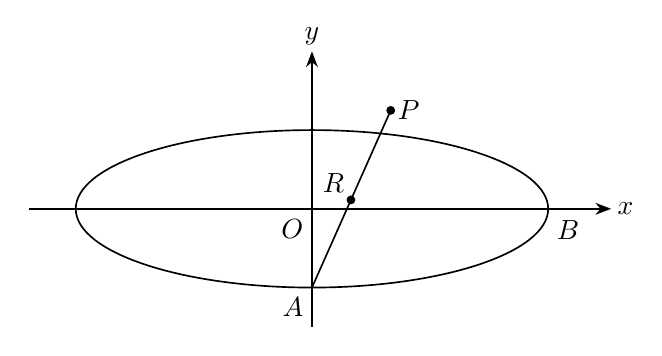
\begin{tikzpicture}[x=1cm,y=1cm,line width=.6pt,font=\normalsize,>=Stealth]
  \coordinate (O) at (0,0);
  \coordinate (A) at (0,-1);
  \coordinate (B) at (3,0);
  \coordinate (P) at (1.0,1.25);
  \coordinate (R) at (0.4948453608,0.1134020619);
  \draw[->] (-3.6,0)--(3.8,0);
  \node[right=2pt,inner sep=0pt] at (3.8,0) {$x$};
  \draw[->] (0,-1.5)--(0,2.0);
  \node[above=2pt,inner sep=0pt] at (0,2.0) {$y$};
  \draw (0,0) ellipse [x radius=3,y radius=1];
  \draw (A)--(P);
  \fill (P) circle (1.6pt);
  \fill (R) circle (1.6pt);
  \node[anchor=north east,inner sep=0pt] at (-0.10,-1.12) {$A$};
  \node[anchor=north west,inner sep=0pt] at (3.10,-0.14) {$B$};
  \node[anchor=north east,inner sep=0pt] at (-0.10,-0.12) {$O$};
  \node[anchor=south east,inner sep=0pt] at (0.42,0.20) {$R$};
  \node[anchor=west,inner sep=0pt] at (1.08,1.25) {$P$};
\end{tikzpicture}
